\documentclass[twoside]{book}

% Packages required by doxygen
\usepackage{fixltx2e}
\usepackage{calc}
\usepackage{doxygen}
\usepackage[export]{adjustbox} % also loads graphicx
\usepackage{graphicx}
\usepackage[utf8]{inputenc}
\usepackage{makeidx}
\usepackage{multicol}
\usepackage{multirow}
\PassOptionsToPackage{warn}{textcomp}
\usepackage{textcomp}
\usepackage[nointegrals]{wasysym}
\usepackage[table]{xcolor}

% Font selection
\usepackage[T1]{fontenc}
\usepackage[scaled=.90]{helvet}
\usepackage{courier}
\usepackage{amssymb}
\usepackage{sectsty}
\renewcommand{\familydefault}{\sfdefault}
\allsectionsfont{%
  \fontseries{bc}\selectfont%
  \color{darkgray}%
}
\renewcommand{\DoxyLabelFont}{%
  \fontseries{bc}\selectfont%
  \color{darkgray}%
}
\newcommand{\+}{\discretionary{\mbox{\scriptsize$\hookleftarrow$}}{}{}}

% Page & text layout
\usepackage{geometry}
\geometry{%
  a4paper,%
  top=2.5cm,%
  bottom=2.5cm,%
  left=2.5cm,%
  right=2.5cm%
}
\tolerance=750
\hfuzz=15pt
\hbadness=750
\setlength{\emergencystretch}{15pt}
\setlength{\parindent}{0cm}
\setlength{\parskip}{3ex plus 2ex minus 2ex}
\makeatletter
\renewcommand{\paragraph}{%
  \@startsection{paragraph}{4}{0ex}{-1.0ex}{1.0ex}{%
    \normalfont\normalsize\bfseries\SS@parafont%
  }%
}
\renewcommand{\subparagraph}{%
  \@startsection{subparagraph}{5}{0ex}{-1.0ex}{1.0ex}{%
    \normalfont\normalsize\bfseries\SS@subparafont%
  }%
}
\makeatother

% Headers & footers
\usepackage{fancyhdr}
\pagestyle{fancyplain}
\fancyhead[LE]{\fancyplain{}{\bfseries\thepage}}
\fancyhead[CE]{\fancyplain{}{}}
\fancyhead[RE]{\fancyplain{}{\bfseries\leftmark}}
\fancyhead[LO]{\fancyplain{}{\bfseries\rightmark}}
\fancyhead[CO]{\fancyplain{}{}}
\fancyhead[RO]{\fancyplain{}{\bfseries\thepage}}
\fancyfoot[LE]{\fancyplain{}{}}
\fancyfoot[CE]{\fancyplain{}{}}
\fancyfoot[RE]{\fancyplain{}{\bfseries\scriptsize Generated by Doxygen }}
\fancyfoot[LO]{\fancyplain{}{\bfseries\scriptsize Generated by Doxygen }}
\fancyfoot[CO]{\fancyplain{}{}}
\fancyfoot[RO]{\fancyplain{}{}}
\renewcommand{\footrulewidth}{0.4pt}
\renewcommand{\chaptermark}[1]{%
  \markboth{#1}{}%
}
\renewcommand{\sectionmark}[1]{%
  \markright{\thesection\ #1}%
}

% Indices & bibliography
\usepackage{natbib}
\usepackage[titles]{tocloft}
\setcounter{tocdepth}{3}
\setcounter{secnumdepth}{5}
\makeindex

% Hyperlinks (required, but should be loaded last)
\usepackage{ifpdf}
\ifpdf
  \usepackage[pdftex,pagebackref=true]{hyperref}
\else
  \usepackage[ps2pdf,pagebackref=true]{hyperref}
\fi
\hypersetup{%
  colorlinks=true,%
  linkcolor=blue,%
  citecolor=blue,%
  unicode%
}

% Custom commands
\newcommand{\clearemptydoublepage}{%
  \newpage{\pagestyle{empty}\cleardoublepage}%
}

\usepackage{caption}
\captionsetup{labelsep=space,justification=centering,font={bf},singlelinecheck=off,skip=4pt,position=top}

%===== C O N T E N T S =====

\begin{document}

% Titlepage & ToC
\hypersetup{pageanchor=false,
             bookmarksnumbered=true,
             pdfencoding=unicode
            }
\pagenumbering{roman}
\begin{titlepage}
\vspace*{7cm}
\begin{center}%
{\Large R\+F\+I\+D\+\_\+keypad\+\_\+lock \\[1ex]\large V1.\+3 }\\
\vspace*{1cm}
{\large Generated by Doxygen 1.8.11}\\
\end{center}
\end{titlepage}
\clearemptydoublepage
\tableofcontents
\clearemptydoublepage
\pagenumbering{arabic}
\hypersetup{pageanchor=true}

%--- Begin generated contents ---
\chapter{Hierarchical Index}
\section{Class Hierarchy}
This inheritance list is sorted roughly, but not completely, alphabetically\+:\begin{DoxyCompactList}
\item \contentsline{section}{access\+Operations}{\pageref{classaccess_operations}}{}
\item \contentsline{section}{matrix\+Keypad}{\pageref{classmatrix_keypad}}{}
\item \contentsline{section}{P\+W\+M\+\_\+signal}{\pageref{class_p_w_m__signal}}{}
\begin{DoxyCompactList}
\item \contentsline{section}{servo}{\pageref{classservo}}{}
\end{DoxyCompactList}
\item \contentsline{section}{R\+F\+ID}{\pageref{class_r_f_i_d}}{}
\begin{DoxyCompactList}
\item \contentsline{section}{mfrc522}{\pageref{classmfrc522}}{}
\end{DoxyCompactList}
\end{DoxyCompactList}

\chapter{Class Index}
\section{Class List}
Here are the classes, structs, unions and interfaces with brief descriptions\+:\begin{DoxyCompactList}
\item\contentsline{section}{\hyperlink{classaccess_operations}{access\+Operations} \\*Operations on accessing the box }{\pageref{classaccess_operations}}{}
\item\contentsline{section}{\hyperlink{classmatrix_keypad}{matrix\+Keypad} \\*Obtain pressed keys from a keypad }{\pageref{classmatrix_keypad}}{}
\item\contentsline{section}{\hyperlink{classmfrc522}{mfrc522} \\*Reading \hyperlink{class_r_f_i_d}{R\+F\+ID} tags with \hyperlink{classmfrc522}{mfrc522} }{\pageref{classmfrc522}}{}
\item\contentsline{section}{\hyperlink{class_p_w_m__signal}{P\+W\+M\+\_\+signal} \\*Basic P\+WM signal }{\pageref{class_p_w_m__signal}}{}
\item\contentsline{section}{\hyperlink{class_r_f_i_d}{R\+F\+ID} \\*\hyperlink{class_r_f_i_d}{R\+F\+ID} superclass }{\pageref{class_r_f_i_d}}{}
\item\contentsline{section}{\hyperlink{classservo}{servo} \\*Servo controll class }{\pageref{classservo}}{}
\end{DoxyCompactList}

\chapter{File Index}
\section{File List}
Here is a list of all documented files with brief descriptions\+:\begin{DoxyCompactList}
\item\contentsline{section}{D\+:/programmeren/\+Projecten/\+I\+P\+A\+S-\/project/rfid\+\_\+keypad\+\_\+lock/\+Finished\+\_\+librarys/{\bfseries access\+Operations.\+hpp} }{\pageref{access_operations_8hpp}}{}
\item\contentsline{section}{D\+:/programmeren/\+Projecten/\+I\+P\+A\+S-\/project/rfid\+\_\+keypad\+\_\+lock/\+Finished\+\_\+librarys/\hyperlink{matrix_keypad_8hpp}{matrix\+Keypad.\+hpp} }{\pageref{matrix_keypad_8hpp}}{}
\item\contentsline{section}{D\+:/programmeren/\+Projecten/\+I\+P\+A\+S-\/project/rfid\+\_\+keypad\+\_\+lock/\+Finished\+\_\+librarys/\hyperlink{mfrc522_8hpp}{mfrc522.\+hpp} }{\pageref{mfrc522_8hpp}}{}
\item\contentsline{section}{D\+:/programmeren/\+Projecten/\+I\+P\+A\+S-\/project/rfid\+\_\+keypad\+\_\+lock/\+Finished\+\_\+librarys/\hyperlink{_p_w_m__signal_8hpp}{P\+W\+M\+\_\+signal.\+hpp} }{\pageref{_p_w_m__signal_8hpp}}{}
\item\contentsline{section}{D\+:/programmeren/\+Projecten/\+I\+P\+A\+S-\/project/rfid\+\_\+keypad\+\_\+lock/\+Finished\+\_\+librarys/\hyperlink{_r_f_i_d_8cpp}{R\+F\+I\+D.\+cpp} }{\pageref{_r_f_i_d_8cpp}}{}
\item\contentsline{section}{D\+:/programmeren/\+Projecten/\+I\+P\+A\+S-\/project/rfid\+\_\+keypad\+\_\+lock/\+Finished\+\_\+librarys/\hyperlink{_r_f_i_d_8hpp}{R\+F\+I\+D.\+hpp} }{\pageref{_r_f_i_d_8hpp}}{}
\item\contentsline{section}{D\+:/programmeren/\+Projecten/\+I\+P\+A\+S-\/project/rfid\+\_\+keypad\+\_\+lock/\+Finished\+\_\+librarys/\hyperlink{servo_8hpp}{servo.\+hpp} }{\pageref{servo_8hpp}}{}
\end{DoxyCompactList}

\chapter{Class Documentation}
\hypertarget{classaccess_operations}{}\section{access\+Operations Class Reference}
\label{classaccess_operations}\index{access\+Operations@{access\+Operations}}


Operations on accessing the box.  




{\ttfamily \#include $<$access\+Operations.\+hpp$>$}

\subsection*{Public Member Functions}
\begin{DoxyCompactItemize}
\item 
\hyperlink{classaccess_operations_a42622d8277e50d7e01118139ab2fd57e}{access\+Operations} (\hyperlink{classmatrix_keypad}{matrix\+Keypad} \&keypad, char $\ast$root\+P\+WD, int len\+Root\+P\+WD, hwlib\+::pin\+\_\+out \&led\+Green=hwlib\+::pin\+\_\+out\+\_\+dummy, hwlib\+::pin\+\_\+out \&led\+Red=hwlib\+::pin\+\_\+out\+\_\+dummy)
\begin{DoxyCompactList}\small\item\em Default constructor. \end{DoxyCompactList}\item 
bool \hyperlink{classaccess_operations_a23a9545b9b8636b995aa6e3d007ea524}{get\+Password} (char $\ast$client\+P\+WD, int len\+Char\+Array)
\begin{DoxyCompactList}\small\item\em Get and check passwords. \end{DoxyCompactList}\item 
bool \hyperlink{classaccess_operations_a93b1c64a9598739a34c09757fe1f4ac1}{set\+Password} (char $\ast$client\+P\+WD, const int \&len\+Char\+Array, int $\ast$current\+Array\+Location)
\begin{DoxyCompactList}\small\item\em Set a new client password. \end{DoxyCompactList}\item 
bool \hyperlink{classaccess_operations_a44956d25fa01c97b6755fbbc30fa7bf7}{check\+Single\+ID} (byte $\ast$ID, int len\+ID, byte $\ast$check\+ID)
\begin{DoxyCompactList}\small\item\em Check one U\+ID. \end{DoxyCompactList}\item 
bool \hyperlink{classaccess_operations_aa1967ef877d37bf37721cde1e41665b0}{check\+Multiple\+ID} (byte $\ast$ID, int len\+ID, int len\+Acces\+I\+Ds, byte($\ast$access\+I\+Ds)\mbox{[}5\mbox{]}, int $\ast$array\+Location)
\begin{DoxyCompactList}\small\item\em Check more than one U\+ID. \end{DoxyCompactList}\end{DoxyCompactItemize}


\subsection{Detailed Description}
Operations on accessing the box. 

This class is meant to make operations on passwords and with passwords a lot more easy. It uses the \hyperlink{classmatrix_keypad}{matrix\+Keypad} library to obtain the passwords. It also contains functions for checking the \hyperlink{class_r_f_i_d}{R\+F\+ID} U\+ID\textquotesingle{}s. 

\subsection{Constructor \& Destructor Documentation}
\index{access\+Operations@{access\+Operations}!access\+Operations@{access\+Operations}}
\index{access\+Operations@{access\+Operations}!access\+Operations@{access\+Operations}}
\subsubsection[{\texorpdfstring{access\+Operations(matrix\+Keypad \&keypad, char $\ast$root\+P\+W\+D, int len\+Root\+P\+W\+D, hwlib\+::pin\+\_\+out \&led\+Green=hwlib\+::pin\+\_\+out\+\_\+dummy, hwlib\+::pin\+\_\+out \&led\+Red=hwlib\+::pin\+\_\+out\+\_\+dummy)}{accessOperations(matrixKeypad &keypad, char *rootPWD, int lenRootPWD, hwlib::pin_out &ledGreen=hwlib::pin_out_dummy, hwlib::pin_out &ledRed=hwlib::pin_out_dummy)}}]{\setlength{\rightskip}{0pt plus 5cm}access\+Operations\+::access\+Operations (
\begin{DoxyParamCaption}
\item[{{\bf matrix\+Keypad} \&}]{keypad, }
\item[{char $\ast$}]{root\+P\+WD, }
\item[{int}]{len\+Root\+P\+WD, }
\item[{hwlib\+::pin\+\_\+out \&}]{led\+Green = {\ttfamily hwlib\+:\+:pin\+\_\+out\+\_\+dummy}, }
\item[{hwlib\+::pin\+\_\+out \&}]{led\+Red = {\ttfamily hwlib\+:\+:pin\+\_\+out\+\_\+dummy}}
\end{DoxyParamCaption}
)}\hypertarget{classaccess_operations_a42622d8277e50d7e01118139ab2fd57e}{}\label{classaccess_operations_a42622d8277e50d7e01118139ab2fd57e}


Default constructor. 

The constructor of this class takes a reference to the matrix keypad to make sure we can use all the functions of the keypad. It also takes a root password meant for changing the user password(s). Two L\+E\+Ds are optional to indicate correct or incorrect passwords and U\+ID\textquotesingle{}s. 

\subsection{Member Function Documentation}
\index{access\+Operations@{access\+Operations}!check\+Multiple\+ID@{check\+Multiple\+ID}}
\index{check\+Multiple\+ID@{check\+Multiple\+ID}!access\+Operations@{access\+Operations}}
\subsubsection[{\texorpdfstring{check\+Multiple\+I\+D(byte $\ast$\+I\+D, int len\+I\+D, int len\+Acces\+I\+Ds, byte($\ast$access\+I\+Ds)[5], int $\ast$array\+Location)}{checkMultipleID(byte *ID, int lenID, int lenAccesIDs, byte(*accessIDs)[5], int *arrayLocation)}}]{\setlength{\rightskip}{0pt plus 5cm}bool access\+Operations\+::check\+Multiple\+ID (
\begin{DoxyParamCaption}
\item[{byte $\ast$}]{ID, }
\item[{int}]{len\+ID, }
\item[{int}]{len\+Acces\+I\+Ds, }
\item[{byte($\ast$)}]{access\+I\+Ds\mbox{[}5\mbox{]}, }
\item[{int $\ast$}]{array\+Location}
\end{DoxyParamCaption}
)}\hypertarget{classaccess_operations_aa1967ef877d37bf37721cde1e41665b0}{}\label{classaccess_operations_aa1967ef877d37bf37721cde1e41665b0}


Check more than one U\+ID. 

The first parameter of this function is the ID that has to be compared to the rest. The length of the ID to compare has to be given as well. The third and fourth parameter are the multidimensional array filled with U\+ID\textquotesingle{}s (or not depending on the amount of users) and the length of that array (first index). The function returns two values. One is a boolean for if statement use and the seccond one is the array location. This location is a parameter that indicates what the index is the ID is found on in the multidimensional array. \index{access\+Operations@{access\+Operations}!check\+Single\+ID@{check\+Single\+ID}}
\index{check\+Single\+ID@{check\+Single\+ID}!access\+Operations@{access\+Operations}}
\subsubsection[{\texorpdfstring{check\+Single\+I\+D(byte $\ast$\+I\+D, int len\+I\+D, byte $\ast$check\+I\+D)}{checkSingleID(byte *ID, int lenID, byte *checkID)}}]{\setlength{\rightskip}{0pt plus 5cm}bool access\+Operations\+::check\+Single\+ID (
\begin{DoxyParamCaption}
\item[{byte $\ast$}]{ID, }
\item[{int}]{len\+ID, }
\item[{byte $\ast$}]{check\+ID}
\end{DoxyParamCaption}
)}\hypertarget{classaccess_operations_a44956d25fa01c97b6755fbbc30fa7bf7}{}\label{classaccess_operations_a44956d25fa01c97b6755fbbc30fa7bf7}


Check one U\+ID. 

This function can be used to check one single U\+ID from an \hyperlink{class_r_f_i_d}{R\+F\+ID} tag. The function requires the ID itself, the length of the ID and the ID to compare the first ID with. It returns true if the 2 ID\textquotesingle{}s match. \index{access\+Operations@{access\+Operations}!get\+Password@{get\+Password}}
\index{get\+Password@{get\+Password}!access\+Operations@{access\+Operations}}
\subsubsection[{\texorpdfstring{get\+Password(char $\ast$client\+P\+W\+D, int len\+Char\+Array)}{getPassword(char *clientPWD, int lenCharArray)}}]{\setlength{\rightskip}{0pt plus 5cm}bool access\+Operations\+::get\+Password (
\begin{DoxyParamCaption}
\item[{char $\ast$}]{client\+P\+WD, }
\item[{int}]{len\+Char\+Array}
\end{DoxyParamCaption}
)}\hypertarget{classaccess_operations_a23a9545b9b8636b995aa6e3d007ea524}{}\label{classaccess_operations_a23a9545b9b8636b995aa6e3d007ea524}


Get and check passwords. 

This function is meant to take a user password and check it against the input it gets from the keypad library. If the input is incorrect it gives you 2 more tries. (for security purposes a long waiting time could be added after 3 wrong tries) The function gives true back if the password was correct and false if the password was incorrect. \index{access\+Operations@{access\+Operations}!set\+Password@{set\+Password}}
\index{set\+Password@{set\+Password}!access\+Operations@{access\+Operations}}
\subsubsection[{\texorpdfstring{set\+Password(char $\ast$client\+P\+W\+D, const int \&len\+Char\+Array, int $\ast$current\+Array\+Location)}{setPassword(char *clientPWD, const int &lenCharArray, int *currentArrayLocation)}}]{\setlength{\rightskip}{0pt plus 5cm}bool access\+Operations\+::set\+Password (
\begin{DoxyParamCaption}
\item[{char $\ast$}]{client\+P\+WD, }
\item[{const int \&}]{len\+Char\+Array, }
\item[{int $\ast$}]{current\+Array\+Location}
\end{DoxyParamCaption}
)}\hypertarget{classaccess_operations_a93b1c64a9598739a34c09757fe1f4ac1}{}\label{classaccess_operations_a93b1c64a9598739a34c09757fe1f4ac1}


Set a new client password. 

This function can be used to change a clients password. It first checks the root password using the \hyperlink{classaccess_operations_a23a9545b9b8636b995aa6e3d007ea524}{get\+Password()} function and if it is correct it will ask you for the new client password. For that is uses the matrix keypad library. If the root password was not filled in correctly the function will return false. If everything word out correctly the function returns true. 

The documentation for this class was generated from the following files\+:\begin{DoxyCompactItemize}
\item 
D\+:/programmeren/\+Projecten/\+I\+P\+A\+S-\/project/rfid\+\_\+keypad\+\_\+lock/\+Finished\+\_\+librarys/access\+Operations.\+hpp\item 
D\+:/programmeren/\+Projecten/\+I\+P\+A\+S-\/project/rfid\+\_\+keypad\+\_\+lock/\+Finished\+\_\+librarys/access\+Operations.\+cpp\end{DoxyCompactItemize}

\hypertarget{classmatrix_keypad}{}\section{matrix\+Keypad Class Reference}
\label{classmatrix_keypad}\index{matrix\+Keypad@{matrix\+Keypad}}


Obtain pressed keys from a keypad.  




{\ttfamily \#include $<$matrix\+Keypad.\+hpp$>$}

\subsection*{Public Member Functions}
\begin{DoxyCompactItemize}
\item 
\hyperlink{classmatrix_keypad_a02a1615e9c24d0d2e1aa939420cf818f}{matrix\+Keypad} (hwlib\+::pin\+\_\+in\+\_\+out \&p0, hwlib\+::pin\+\_\+in\+\_\+out \&p1, hwlib\+::pin\+\_\+in\+\_\+out \&p2, hwlib\+::pin\+\_\+in\+\_\+out \&p3, hwlib\+::pin\+\_\+in\+\_\+out \&p4, hwlib\+::pin\+\_\+in\+\_\+out \&p5, hwlib\+::pin\+\_\+in\+\_\+out \&p6, hwlib\+::pin\+\_\+in\+\_\+out \&p7=hwlib\+::pin\+\_\+in\+\_\+out\+\_\+dummy, int col\+Size=3, hwlib\+::pin\+\_\+out \&buzzer\+Pin=hwlib\+::pin\+\_\+out\+\_\+dummy)
\begin{DoxyCompactList}\small\item\em Default constructor. \end{DoxyCompactList}\item 
char \hyperlink{classmatrix_keypad_adb0562ac12409dd390afe759297d7a95}{get\+Key} ()
\begin{DoxyCompactList}\small\item\em Obtain seperate keys. \end{DoxyCompactList}\item 
int \hyperlink{classmatrix_keypad_a85cb23086207b678f0a64f160d607c5d}{get\+String} (char $\ast$chararray, int len\+Char\+Array)
\begin{DoxyCompactList}\small\item\em Obtain a string. \end{DoxyCompactList}\end{DoxyCompactItemize}


\subsection{Detailed Description}
Obtain pressed keys from a keypad. 

This is a class that can be used to obtain pressed keys from a keypad using an Arduino Due board. The seperate keypresses can be obtained or an array of characters can be filled with pressed characters. It uses another namespace containing classes that make it capable of using Arduino Due pins. This second namespace has been made by Wouter Ooijen and not by me. 

\subsection{Constructor \& Destructor Documentation}
\index{matrix\+Keypad@{matrix\+Keypad}!matrix\+Keypad@{matrix\+Keypad}}
\index{matrix\+Keypad@{matrix\+Keypad}!matrix\+Keypad@{matrix\+Keypad}}
\subsubsection[{\texorpdfstring{matrix\+Keypad(hwlib\+::pin\+\_\+in\+\_\+out \&p0, hwlib\+::pin\+\_\+in\+\_\+out \&p1, hwlib\+::pin\+\_\+in\+\_\+out \&p2, hwlib\+::pin\+\_\+in\+\_\+out \&p3, hwlib\+::pin\+\_\+in\+\_\+out \&p4, hwlib\+::pin\+\_\+in\+\_\+out \&p5, hwlib\+::pin\+\_\+in\+\_\+out \&p6, hwlib\+::pin\+\_\+in\+\_\+out \&p7=hwlib\+::pin\+\_\+in\+\_\+out\+\_\+dummy, int col\+Size=3, hwlib\+::pin\+\_\+out \&buzzer\+Pin=hwlib\+::pin\+\_\+out\+\_\+dummy)}{matrixKeypad(hwlib::pin_in_out &p0, hwlib::pin_in_out &p1, hwlib::pin_in_out &p2, hwlib::pin_in_out &p3, hwlib::pin_in_out &p4, hwlib::pin_in_out &p5, hwlib::pin_in_out &p6, hwlib::pin_in_out &p7=hwlib::pin_in_out_dummy, int colSize=3, hwlib::pin_out &buzzerPin=hwlib::pin_out_dummy)}}]{\setlength{\rightskip}{0pt plus 5cm}matrix\+Keypad\+::matrix\+Keypad (
\begin{DoxyParamCaption}
\item[{hwlib\+::pin\+\_\+in\+\_\+out \&}]{p0, }
\item[{hwlib\+::pin\+\_\+in\+\_\+out \&}]{p1, }
\item[{hwlib\+::pin\+\_\+in\+\_\+out \&}]{p2, }
\item[{hwlib\+::pin\+\_\+in\+\_\+out \&}]{p3, }
\item[{hwlib\+::pin\+\_\+in\+\_\+out \&}]{p4, }
\item[{hwlib\+::pin\+\_\+in\+\_\+out \&}]{p5, }
\item[{hwlib\+::pin\+\_\+in\+\_\+out \&}]{p6, }
\item[{hwlib\+::pin\+\_\+in\+\_\+out \&}]{p7 = {\ttfamily hwlib\+:\+:pin\+\_\+in\+\_\+out\+\_\+dummy}, }
\item[{int}]{col\+Size = {\ttfamily 3}, }
\item[{hwlib\+::pin\+\_\+out \&}]{buzzer\+Pin = {\ttfamily hwlib\+:\+:pin\+\_\+out\+\_\+dummy}}
\end{DoxyParamCaption}
)}\hypertarget{classmatrix_keypad_a02a1615e9c24d0d2e1aa939420cf818f}{}\label{classmatrix_keypad_a02a1615e9c24d0d2e1aa939420cf818f}


Default constructor. 

This constructor sets up all the pins on the Arduino Due. It takes the size of the keypad and the pins on wich it is attached. The last pin is setup with a dummy as default value to ensure that 4x3 keypads dont give errors. It als takes a buzzerpin for giving a little sound when a key is pressed. This pin also has a dummy as default. This makes sure the buzzer is not actually needed. 

\subsection{Member Function Documentation}
\index{matrix\+Keypad@{matrix\+Keypad}!get\+Key@{get\+Key}}
\index{get\+Key@{get\+Key}!matrix\+Keypad@{matrix\+Keypad}}
\subsubsection[{\texorpdfstring{get\+Key()}{getKey()}}]{\setlength{\rightskip}{0pt plus 5cm}char matrix\+Keypad\+::get\+Key (
\begin{DoxyParamCaption}
{}
\end{DoxyParamCaption}
)}\hypertarget{classmatrix_keypad_adb0562ac12409dd390afe759297d7a95}{}\label{classmatrix_keypad_adb0562ac12409dd390afe759297d7a95}


Obtain seperate keys. 

This function optains the seperate keys from the keypad. It waits for a key to be pressed and then returns the pressed key as an character. It knows what key was pressed by seting up 4 inputs and 4(or 3) outputs. The inputs have a pullup resistor. After that it checks for a row that is pulled down to 0. After that it has the pressed row. To know the pressed column, it switches the inputs to outputs and the outputs to inputs. That way it can check the pressed column. \index{matrix\+Keypad@{matrix\+Keypad}!get\+String@{get\+String}}
\index{get\+String@{get\+String}!matrix\+Keypad@{matrix\+Keypad}}
\subsubsection[{\texorpdfstring{get\+String(char $\ast$chararray, int len\+Char\+Array)}{getString(char *chararray, int lenCharArray)}}]{\setlength{\rightskip}{0pt plus 5cm}int matrix\+Keypad\+::get\+String (
\begin{DoxyParamCaption}
\item[{char $\ast$}]{chararray, }
\item[{int}]{len\+Char\+Array}
\end{DoxyParamCaption}
)}\hypertarget{classmatrix_keypad_a85cb23086207b678f0a64f160d607c5d}{}\label{classmatrix_keypad_a85cb23086207b678f0a64f160d607c5d}


Obtain a string. 

This function uses the \hyperlink{classmatrix_keypad_adb0562ac12409dd390afe759297d7a95}{get\+Key()} function to obtain the seperate keys. It puts these pressed keys in a user defined array with a user defined array length. If the maximum length of the array -\/1 (for the \textquotesingle{}\textbackslash{}0\textquotesingle{} character) has been reached, it protects you from going out of the array. To stop with getting characters before the array is full you have to press the \textquotesingle{}\#\textquotesingle{} character. This will stops the process and adds a \textquotesingle{}\textbackslash{}0\textquotesingle{} after the last character. The function returns the array size usable with for loops to go through the array and execute operations on the array. 

The documentation for this class was generated from the following files\+:\begin{DoxyCompactItemize}
\item 
D\+:/programmeren/\+Projecten/\+I\+P\+A\+S-\/project/rfid\+\_\+keypad\+\_\+lock/\+Finished\+\_\+librarys/\hyperlink{matrix_keypad_8hpp}{matrix\+Keypad.\+hpp}\item 
D\+:/programmeren/\+Projecten/\+I\+P\+A\+S-\/project/rfid\+\_\+keypad\+\_\+lock/\+Finished\+\_\+librarys/matrix\+Keypad.\+cpp\end{DoxyCompactItemize}

\hypertarget{classmfrc522}{}\section{mfrc522 Class Reference}
\label{classmfrc522}\index{mfrc522@{mfrc522}}


Reading \hyperlink{class_r_f_i_d}{R\+F\+ID} tags with \hyperlink{classmfrc522}{mfrc522}.  




{\ttfamily \#include $<$mfrc522.\+hpp$>$}

Inheritance diagram for mfrc522\+:\begin{figure}[H]
\begin{center}
\leavevmode
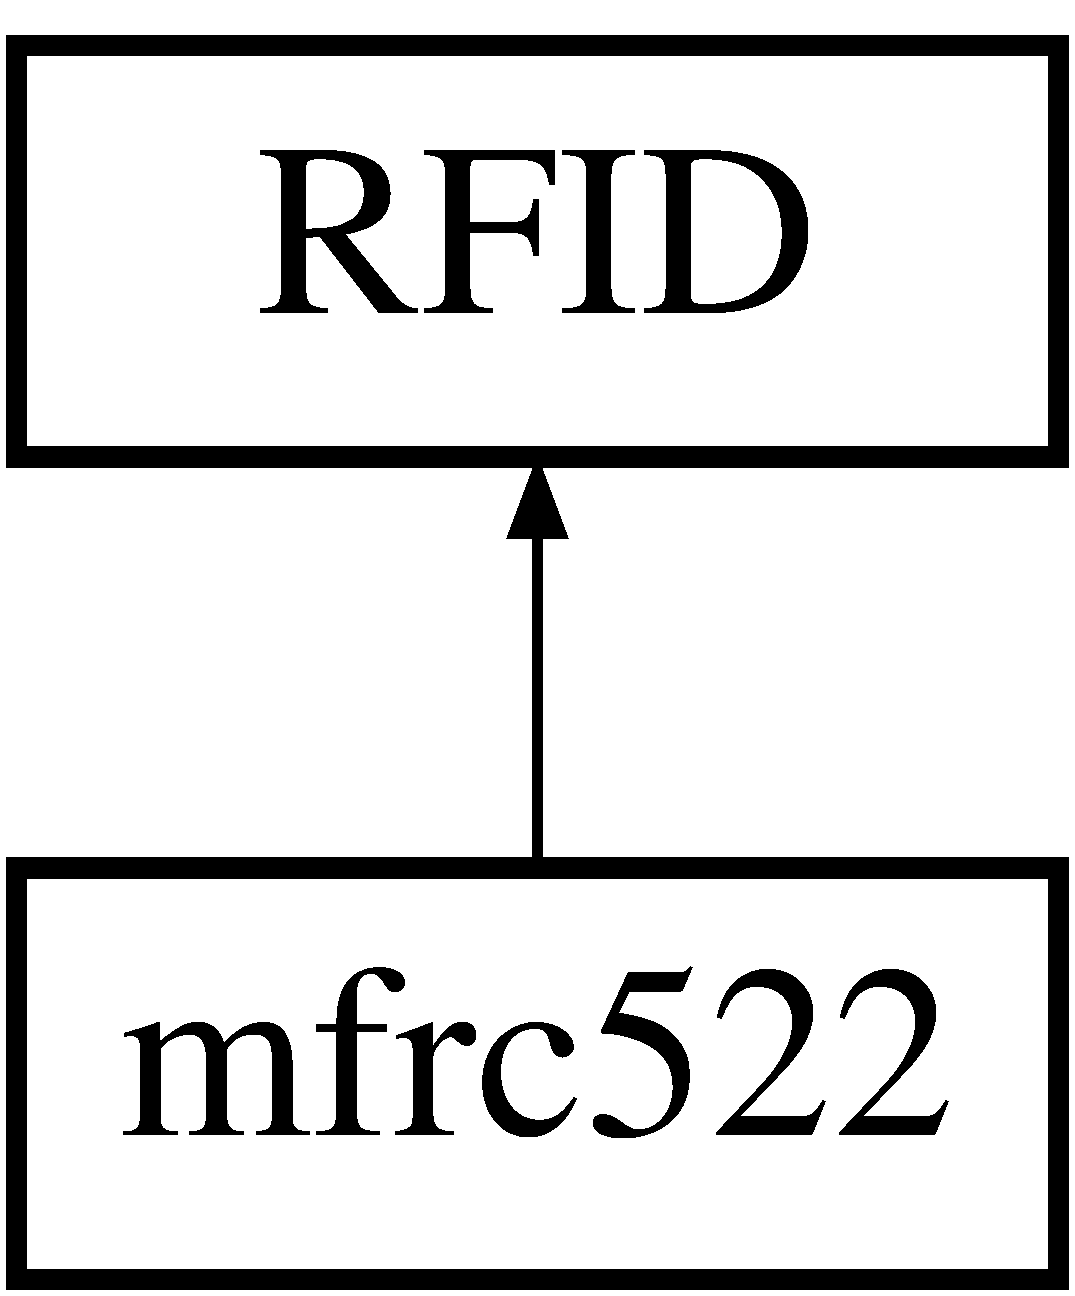
\includegraphics[height=2.000000cm]{classmfrc522}
\end{center}
\end{figure}
\subsection*{Public Member Functions}
\begin{DoxyCompactItemize}
\item 
\hyperlink{classmfrc522_a7939e9c2b9c197a409489af7fe3c9da7}{mfrc522} (hwlib\+::spi\+\_\+bus\+\_\+bit\+\_\+banged\+\_\+sclk\+\_\+mosi\+\_\+miso \&spi, hwlib\+::target\+::pin\+\_\+out \&S\+DA, hwlib\+::target\+::pin\+\_\+out \&R\+E\+S\+ET)
\begin{DoxyCompactList}\small\item\em Default constructor. \end{DoxyCompactList}\item 
void \hyperlink{classmfrc522_ac0a0cf7f16b98c37826ce0e160877269}{init} () override
\begin{DoxyCompactList}\small\item\em Initialization of the \hyperlink{classmfrc522}{mfrc522}. \end{DoxyCompactList}\item 
void \hyperlink{classmfrc522_a7b93914a7f2e1fd587392c2949f16ab1}{antenna\+On} ()
\begin{DoxyCompactList}\small\item\em Turn the antenna on. \end{DoxyCompactList}\item 
byte \hyperlink{classmfrc522_a0e19de4c39b37cf31d45af78f0fad524}{request} (byte mode, byte $\ast$back\+Data)
\begin{DoxyCompactList}\small\item\em Send data request. \end{DoxyCompactList}\item 
void \hyperlink{classmfrc522_a6801b8481392f6310b40a6893f6544c2}{to\+Card} (byte value, byte $\ast$send\+Data, int len\+Send\+Data, byte $\ast$card\+Ret\+Value, byte $\ast$back\+Data) override
\begin{DoxyCompactList}\small\item\em Send data to the \hyperlink{class_r_f_i_d}{R\+F\+ID} tag and get the returned information. \end{DoxyCompactList}\item 
byte \hyperlink{classmfrc522_a0ecbb86c1ad7fe15ea404f5bd8f30297}{anticoll} (byte $\ast$back\+Data)
\begin{DoxyCompactList}\small\item\em Check for collision and return the U\+ID. \end{DoxyCompactList}\item 
void \hyperlink{classmfrc522_a18665350caf822a716f2a72674a21647}{wait\+For\+Card\+ID} (byte $\ast$ID, int len\+ID) override
\begin{DoxyCompactList}\small\item\em Wait for a tag to be found and read it. \end{DoxyCompactList}\end{DoxyCompactItemize}
\subsection*{Public Attributes}
\begin{DoxyCompactItemize}
\item 
int {\bfseries M\+A\+X\+\_\+\+L\+EN} = 16\hypertarget{classmfrc522_ab5aeddf4462b8cbd6d4979a5aa591e2a}{}\label{classmfrc522_ab5aeddf4462b8cbd6d4979a5aa591e2a}

\item 
const byte {\bfseries I\+D\+LE} = 0\+X00\hypertarget{classmfrc522_a2db7d04e72f02ce2cd1d2f3c2a142d9b}{}\label{classmfrc522_a2db7d04e72f02ce2cd1d2f3c2a142d9b}

\item 
const byte {\bfseries T\+R\+A\+N\+S\+C\+E\+I\+VE} = 0x0C\hypertarget{classmfrc522_a4265ed9beb2068796f558866ecb7d599}{}\label{classmfrc522_a4265ed9beb2068796f558866ecb7d599}

\item 
const byte {\bfseries S\+O\+F\+T\+R\+E\+S\+ET} = 0x0F\hypertarget{classmfrc522_a5636b5a1e9382e1cc842fa20723d63bb}{}\label{classmfrc522_a5636b5a1e9382e1cc842fa20723d63bb}

\item 
const byte {\bfseries M\+F\+A\+U\+T\+H\+E\+NT} = 0x0E\hypertarget{classmfrc522_a65673200cf51c637d3998187b747f642}{}\label{classmfrc522_a65673200cf51c637d3998187b747f642}

\item 
const byte {\bfseries A\+N\+T\+I\+C\+O\+LL} = 0\+X93\hypertarget{classmfrc522_a19f4e763eb734d352e9c0bf4694030b1}{}\label{classmfrc522_a19f4e763eb734d352e9c0bf4694030b1}

\item 
const byte {\bfseries R\+E\+Q\+I\+DL} = 0x26\hypertarget{classmfrc522_ad0ab76f65c6fff489ac36b763e588e17}{}\label{classmfrc522_ad0ab76f65c6fff489ac36b763e588e17}

\item 
const byte {\bfseries M\+I\+\_\+\+OK} = 0\hypertarget{classmfrc522_ae9691458db3d46de5632ef531c0a06bc}{}\label{classmfrc522_ae9691458db3d46de5632ef531c0a06bc}

\item 
const byte {\bfseries M\+I\+\_\+\+N\+O\+T\+A\+G\+E\+RR} = 1\hypertarget{classmfrc522_abcdae51991b17be0222a25c351f36c08}{}\label{classmfrc522_abcdae51991b17be0222a25c351f36c08}

\item 
const byte {\bfseries M\+I\+\_\+\+E\+RR} = 2\hypertarget{classmfrc522_a6a308a9c089dea6dbab9366fc939c313}{}\label{classmfrc522_a6a308a9c089dea6dbab9366fc939c313}

\item 
const byte {\bfseries Command\+Reg} = ((0x01 $<$$<$ 1) \& 0x7\+E)\hypertarget{classmfrc522_abc418205b4d996c1541bfda1ce89c196}{}\label{classmfrc522_abc418205b4d996c1541bfda1ce89c196}

\item 
const byte {\bfseries F\+I\+F\+O\+Data\+Reg} = ((0x09 $<$$<$ 1) \& 0\+X7\+E)\hypertarget{classmfrc522_aa1dd9bd0fb405bc8217cc6c655c0b434}{}\label{classmfrc522_aa1dd9bd0fb405bc8217cc6c655c0b434}

\item 
const byte {\bfseries T\+Mode\+Reg} = ((0x2\+A $<$$<$ 1) \& 0\+X7\+E)\hypertarget{classmfrc522_ab4ce527983527c3db68f7541cb6b62fc}{}\label{classmfrc522_ab4ce527983527c3db68f7541cb6b62fc}

\item 
const byte {\bfseries T\+Prescaler\+Reg} = ((0x2\+B $<$$<$ 1) \& 0\+X7\+E)\hypertarget{classmfrc522_a1b54b9b1e82ebc217c280928d1f567f1}{}\label{classmfrc522_a1b54b9b1e82ebc217c280928d1f567f1}

\item 
const byte {\bfseries T\+Reload\+RegH} = ((0x2\+C $<$$<$ 1) \& 0\+X7\+E)\hypertarget{classmfrc522_a491eb14159868a7aaf5c0d23ea5679f5}{}\label{classmfrc522_a491eb14159868a7aaf5c0d23ea5679f5}

\item 
const byte {\bfseries T\+Reload\+RegL} = ((0x2\+D $<$$<$ 1) \& 0\+X7\+E)\hypertarget{classmfrc522_a1bfa3adaddcb782565d871c0efed53d1}{}\label{classmfrc522_a1bfa3adaddcb782565d871c0efed53d1}

\item 
const byte {\bfseries Tx\+A\+S\+K\+Reg} = ((0x15 $<$$<$ 1) \& 0\+X7\+E)\hypertarget{classmfrc522_a365974a47e52e69d7008df3b37019ecd}{}\label{classmfrc522_a365974a47e52e69d7008df3b37019ecd}

\item 
const byte {\bfseries Mode\+Reg} = ((0x11 $<$$<$ 1) \& 0\+X7\+E)\hypertarget{classmfrc522_a89d0eb6565c3c0c37dfde546f4cab24f}{}\label{classmfrc522_a89d0eb6565c3c0c37dfde546f4cab24f}

\item 
const byte {\bfseries Tx\+Control\+Reg} = ((0x14 $<$$<$ 1) \& 0\+X7\+E)\hypertarget{classmfrc522_a50e31c19c5289374ea3f8e397b30ae5a}{}\label{classmfrc522_a50e31c19c5289374ea3f8e397b30ae5a}

\item 
const byte {\bfseries Bit\+Framing\+Reg} = ((0x0\+D $<$$<$ 1) \& 0x7\+E)\hypertarget{classmfrc522_a1147f52a011b9cf58a3bfe39886bfa55}{}\label{classmfrc522_a1147f52a011b9cf58a3bfe39886bfa55}

\item 
const byte {\bfseries Com\+I\+En\+Reg} = ((0x02 $<$$<$ 1) \& 0x7\+E)\hypertarget{classmfrc522_a746894aa1857a071ab9573ecf07621a0}{}\label{classmfrc522_a746894aa1857a071ab9573ecf07621a0}

\item 
const byte {\bfseries Com\+Irq\+Reg} = ((0x04 $<$$<$ 1) \& 0x7\+E)\hypertarget{classmfrc522_a4fb04a221dc26dee599d32119eebe0cc}{}\label{classmfrc522_a4fb04a221dc26dee599d32119eebe0cc}

\item 
const byte {\bfseries F\+I\+F\+O\+Level\+Reg} = ((0x0\+A $<$$<$ 1) \& 0x7\+E)\hypertarget{classmfrc522_a75a41a00f61652eec99c887d98df8ed4}{}\label{classmfrc522_a75a41a00f61652eec99c887d98df8ed4}

\item 
const byte {\bfseries Error\+Reg} = ((0x06 $<$$<$ 1) \& 0x7\+E)\hypertarget{classmfrc522_a91f4e4c517d9f583250a6f5b022c590d}{}\label{classmfrc522_a91f4e4c517d9f583250a6f5b022c590d}

\item 
const byte {\bfseries Control\+Reg} = ((0x0\+C $<$$<$ 1) \& 0x7\+E)\hypertarget{classmfrc522_ad2e13b4fb8a39ed0200b467666266346}{}\label{classmfrc522_ad2e13b4fb8a39ed0200b467666266346}

\end{DoxyCompactItemize}
\subsection*{Additional Inherited Members}


\subsection{Detailed Description}
Reading \hyperlink{class_r_f_i_d}{R\+F\+ID} tags with \hyperlink{classmfrc522}{mfrc522}. 

This class can be used to read the U\+ID of an \hyperlink{class_r_f_i_d}{R\+F\+ID} tag. It uses another set of classes created by Wouter van Ooijen. The other classes are used for reading from and writing values to the G\+P\+IO pins on the Arduino Due. This library is a recreation from a python original that can be found on this link\+: \href{https://github.com/mxgxw/MFRC522-python}{\tt https\+://github.\+com/mxgxw/\+M\+F\+R\+C522-\/python}. 

\subsection{Constructor \& Destructor Documentation}
\index{mfrc522@{mfrc522}!mfrc522@{mfrc522}}
\index{mfrc522@{mfrc522}!mfrc522@{mfrc522}}
\subsubsection[{\texorpdfstring{mfrc522(hwlib\+::spi\+\_\+bus\+\_\+bit\+\_\+banged\+\_\+sclk\+\_\+mosi\+\_\+miso \&spi, hwlib\+::target\+::pin\+\_\+out \&\+S\+D\+A, hwlib\+::target\+::pin\+\_\+out \&\+R\+E\+S\+E\+T)}{mfrc522(hwlib::spi_bus_bit_banged_sclk_mosi_miso &spi, hwlib::target::pin_out &SDA, hwlib::target::pin_out &RESET)}}]{\setlength{\rightskip}{0pt plus 5cm}mfrc522\+::mfrc522 (
\begin{DoxyParamCaption}
\item[{hwlib\+::spi\+\_\+bus\+\_\+bit\+\_\+banged\+\_\+sclk\+\_\+mosi\+\_\+miso \&}]{spi, }
\item[{hwlib\+::target\+::pin\+\_\+out \&}]{S\+DA, }
\item[{hwlib\+::target\+::pin\+\_\+out \&}]{R\+E\+S\+ET}
\end{DoxyParamCaption}
)}\hypertarget{classmfrc522_a7939e9c2b9c197a409489af7fe3c9da7}{}\label{classmfrc522_a7939e9c2b9c197a409489af7fe3c9da7}


Default constructor. 

The constructor takes three items from the hwlib namespace, the already created spi interface, the ss or chip select line that is attached to the S\+DA pin of the \hyperlink{classmfrc522}{mfrc522} and the R\+E\+S\+ET pin. The R\+E\+S\+ET pin is for hard resetting the \hyperlink{classmfrc522}{mfrc522}. 

\subsection{Member Function Documentation}
\index{mfrc522@{mfrc522}!antenna\+On@{antenna\+On}}
\index{antenna\+On@{antenna\+On}!mfrc522@{mfrc522}}
\subsubsection[{\texorpdfstring{antenna\+On()}{antennaOn()}}]{\setlength{\rightskip}{0pt plus 5cm}void mfrc522\+::antenna\+On (
\begin{DoxyParamCaption}
{}
\end{DoxyParamCaption}
)}\hypertarget{classmfrc522_a7b93914a7f2e1fd587392c2949f16ab1}{}\label{classmfrc522_a7b93914a7f2e1fd587392c2949f16ab1}


Turn the antenna on. 

After a softreset the antenna for reading the \hyperlink{class_r_f_i_d}{R\+F\+ID} tags is turned off. To turn it on we have the antenna\+On function. It reads the Tx\+Control\+Register and checks the returned value to see if the antenna is still on. If it is not on the set\+Bit\+Mask function turns it on. \index{mfrc522@{mfrc522}!anticoll@{anticoll}}
\index{anticoll@{anticoll}!mfrc522@{mfrc522}}
\subsubsection[{\texorpdfstring{anticoll(byte $\ast$back\+Data)}{anticoll(byte *backData)}}]{\setlength{\rightskip}{0pt plus 5cm}byte mfrc522\+::anticoll (
\begin{DoxyParamCaption}
\item[{byte $\ast$}]{back\+Data}
\end{DoxyParamCaption}
)}\hypertarget{classmfrc522_a0ecbb86c1ad7fe15ea404f5bd8f30297}{}\label{classmfrc522_a0ecbb86c1ad7fe15ea404f5bd8f30297}


Check for collision and return the U\+ID. 

This function checks for collision errors and returns the U\+ID of a tag. The return value is a byte that shows the status. If the return value is equal to M\+I\+\_\+\+E\+RR or M\+I\+\_\+\+N\+O\+T\+A\+G\+E\+RR then something went wrong. The data it returns is 5 bytes long. \index{mfrc522@{mfrc522}!init@{init}}
\index{init@{init}!mfrc522@{mfrc522}}
\subsubsection[{\texorpdfstring{init() override}{init() override}}]{\setlength{\rightskip}{0pt plus 5cm}void mfrc522\+::init (
\begin{DoxyParamCaption}
{}
\end{DoxyParamCaption}
)\hspace{0.3cm}{\ttfamily [override]}, {\ttfamily [virtual]}}\hypertarget{classmfrc522_ac0a0cf7f16b98c37826ce0e160877269}{}\label{classmfrc522_ac0a0cf7f16b98c37826ce0e160877269}


Initialization of the \hyperlink{classmfrc522}{mfrc522}. 

This function contains al the setting that are needed to be done for the \hyperlink{classmfrc522}{mfrc522} to send the correct information. It is beeing called by the constructor automatically when the constructor is beeing called. For more information about the different settings, check the cpp file. Comments have been added to every line that send something to the \hyperlink{classmfrc522}{mfrc522}. 

Implements \hyperlink{class_r_f_i_d_a8b244d38edcafaeb06637dbf33b5656f}{R\+F\+ID}.

\index{mfrc522@{mfrc522}!request@{request}}
\index{request@{request}!mfrc522@{mfrc522}}
\subsubsection[{\texorpdfstring{request(byte mode, byte $\ast$back\+Data)}{request(byte mode, byte *backData)}}]{\setlength{\rightskip}{0pt plus 5cm}byte mfrc522\+::request (
\begin{DoxyParamCaption}
\item[{byte}]{mode, }
\item[{byte $\ast$}]{back\+Data}
\end{DoxyParamCaption}
)}\hypertarget{classmfrc522_a0e19de4c39b37cf31d45af78f0fad524}{}\label{classmfrc522_a0e19de4c39b37cf31d45af78f0fad524}


Send data request. 

This function sends a data request to the \hyperlink{class_r_f_i_d}{R\+F\+ID} tag. If we get M\+I\+\_\+\+OK back and the length of the return data of the tag is equal to 0x10 (in bits), we can start getting the U\+ID data. That is done by the anticoll function. This function returns the status. \index{mfrc522@{mfrc522}!to\+Card@{to\+Card}}
\index{to\+Card@{to\+Card}!mfrc522@{mfrc522}}
\subsubsection[{\texorpdfstring{to\+Card(byte value, byte $\ast$send\+Data, int len\+Send\+Data, byte $\ast$card\+Ret\+Value, byte $\ast$back\+Data) override}{toCard(byte value, byte *sendData, int lenSendData, byte *cardRetValue, byte *backData) override}}]{\setlength{\rightskip}{0pt plus 5cm}void mfrc522\+::to\+Card (
\begin{DoxyParamCaption}
\item[{byte}]{value, }
\item[{byte $\ast$}]{send\+Data, }
\item[{int}]{len\+Send\+Data, }
\item[{byte $\ast$}]{card\+Ret\+Value, }
\item[{byte $\ast$}]{back\+Data}
\end{DoxyParamCaption}
)\hspace{0.3cm}{\ttfamily [override]}, {\ttfamily [virtual]}}\hypertarget{classmfrc522_a6801b8481392f6310b40a6893f6544c2}{}\label{classmfrc522_a6801b8481392f6310b40a6893f6544c2}


Send data to the \hyperlink{class_r_f_i_d}{R\+F\+ID} tag and get the returned information. 

We send data to the \hyperlink{class_r_f_i_d}{R\+F\+ID} tag and get the return data back from the tag. The data that comes back is beeing returned using the card\+Ret\+Value and back\+Data parameters. back\+Data contains the bytes of data returned by the tag. card\+Ret\+Value contains the status and the length of the returned data. 

Implements \hyperlink{class_r_f_i_d_ad44955169cde018c9673ae5073fcac24}{R\+F\+ID}.

\index{mfrc522@{mfrc522}!wait\+For\+Card\+ID@{wait\+For\+Card\+ID}}
\index{wait\+For\+Card\+ID@{wait\+For\+Card\+ID}!mfrc522@{mfrc522}}
\subsubsection[{\texorpdfstring{wait\+For\+Card\+I\+D(byte $\ast$\+I\+D, int len\+I\+D) override}{waitForCardID(byte *ID, int lenID) override}}]{\setlength{\rightskip}{0pt plus 5cm}void mfrc522\+::wait\+For\+Card\+ID (
\begin{DoxyParamCaption}
\item[{byte $\ast$}]{ID, }
\item[{int}]{len\+ID}
\end{DoxyParamCaption}
)\hspace{0.3cm}{\ttfamily [override]}, {\ttfamily [virtual]}}\hypertarget{classmfrc522_a18665350caf822a716f2a72674a21647}{}\label{classmfrc522_a18665350caf822a716f2a72674a21647}


Wait for a tag to be found and read it. 

This function waits for a new \hyperlink{class_r_f_i_d}{R\+F\+ID} tag to be found. If it is found the function reads the U\+ID of the tag. The function returns the U\+ID. using a ID parameter on the function call. This ID parameter is a byte array that is 5 bytes long. Notice\+: the function dus not have an actual return value, it uses the ID parameter to return the U\+ID. 

Implements \hyperlink{class_r_f_i_d_a7e02863bc0f1f117b05d72f9063497f7}{R\+F\+ID}.



The documentation for this class was generated from the following files\+:\begin{DoxyCompactItemize}
\item 
\hyperlink{mfrc522_8hpp}{mfrc522.\+hpp}\item 
mfrc522.\+cpp\end{DoxyCompactItemize}

\hypertarget{class_p_w_m__signal}{}\section{P\+W\+M\+\_\+signal Class Reference}
\label{class_p_w_m__signal}\index{P\+W\+M\+\_\+signal@{P\+W\+M\+\_\+signal}}


Basic P\+WM signal.  




{\ttfamily \#include $<$P\+W\+M\+\_\+signal.\+hpp$>$}

Inheritance diagram for P\+W\+M\+\_\+signal\+:\begin{figure}[H]
\begin{center}
\leavevmode
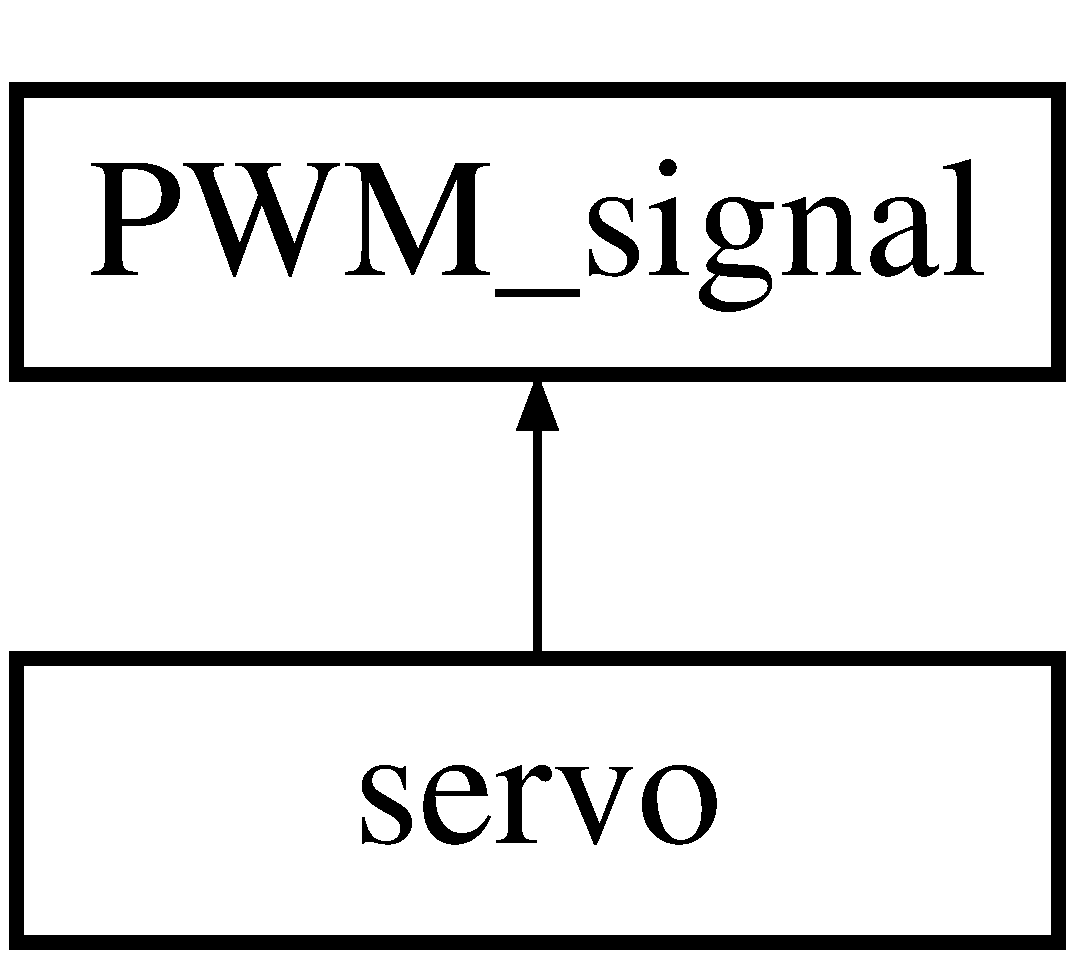
\includegraphics[height=2.000000cm]{class_p_w_m__signal}
\end{center}
\end{figure}
\subsection*{Public Member Functions}
\begin{DoxyCompactItemize}
\item 
\hyperlink{class_p_w_m__signal_ad64aad0e6fe9cf246715bc9cf0f78247}{P\+W\+M\+\_\+signal} (hwlib\+::target\+::pin\+\_\+out \&pwm\+Pin)
\begin{DoxyCompactList}\small\item\em The pin to wich the P\+WM device has been attached. \end{DoxyCompactList}\item 
void \hyperlink{class_p_w_m__signal_a82a9e4648b24a15992b59918e640157c}{P\+W\+M\+\_\+pulse} (int pulse\+Width)
\begin{DoxyCompactList}\small\item\em One pulse. \end{DoxyCompactList}\end{DoxyCompactItemize}


\subsection{Detailed Description}
Basic P\+WM signal. 

This class is for creating a basic P\+WN signal object and then call seperate pules with a certain pulsewidth. It uses a bit banged version of P\+WM. 

\subsection{Constructor \& Destructor Documentation}
\index{P\+W\+M\+\_\+signal@{P\+W\+M\+\_\+signal}!P\+W\+M\+\_\+signal@{P\+W\+M\+\_\+signal}}
\index{P\+W\+M\+\_\+signal@{P\+W\+M\+\_\+signal}!P\+W\+M\+\_\+signal@{P\+W\+M\+\_\+signal}}
\subsubsection[{\texorpdfstring{P\+W\+M\+\_\+signal(hwlib\+::target\+::pin\+\_\+out \&pwm\+Pin)}{PWM_signal(hwlib::target::pin_out &pwmPin)}}]{\setlength{\rightskip}{0pt plus 5cm}P\+W\+M\+\_\+signal\+::\+P\+W\+M\+\_\+signal (
\begin{DoxyParamCaption}
\item[{hwlib\+::target\+::pin\+\_\+out \&}]{pwm\+Pin}
\end{DoxyParamCaption}
)}\hypertarget{class_p_w_m__signal_ad64aad0e6fe9cf246715bc9cf0f78247}{}\label{class_p_w_m__signal_ad64aad0e6fe9cf246715bc9cf0f78247}


The pin to wich the P\+WM device has been attached. 

Default constructor This constructor sets up a pin to control using pwm. It does this using the pin\+\_\+out class in namespace hwlib. 

\subsection{Member Function Documentation}
\index{P\+W\+M\+\_\+signal@{P\+W\+M\+\_\+signal}!P\+W\+M\+\_\+pulse@{P\+W\+M\+\_\+pulse}}
\index{P\+W\+M\+\_\+pulse@{P\+W\+M\+\_\+pulse}!P\+W\+M\+\_\+signal@{P\+W\+M\+\_\+signal}}
\subsubsection[{\texorpdfstring{P\+W\+M\+\_\+pulse(int pulse\+Width)}{PWM_pulse(int pulseWidth)}}]{\setlength{\rightskip}{0pt plus 5cm}void P\+W\+M\+\_\+signal\+::\+P\+W\+M\+\_\+pulse (
\begin{DoxyParamCaption}
\item[{int}]{pulse\+Width}
\end{DoxyParamCaption}
)}\hypertarget{class_p_w_m__signal_a82a9e4648b24a15992b59918e640157c}{}\label{class_p_w_m__signal_a82a9e4648b24a15992b59918e640157c}


One pulse. 

This function is made to create one P\+WM pulse with a user specified pulsewidth. The wait time between every pulse is about 20 ms. 

The documentation for this class was generated from the following files\+:\begin{DoxyCompactItemize}
\item 
D\+:/programmeren/\+Projecten/\+I\+P\+A\+S-\/project/rfid\+\_\+keypad\+\_\+lock/\+Finished\+\_\+librarys/\hyperlink{_p_w_m__signal_8hpp}{P\+W\+M\+\_\+signal.\+hpp}\item 
D\+:/programmeren/\+Projecten/\+I\+P\+A\+S-\/project/rfid\+\_\+keypad\+\_\+lock/\+Finished\+\_\+librarys/P\+W\+M\+\_\+signal.\+cpp\end{DoxyCompactItemize}

\hypertarget{class_r_f_i_d}{}\section{R\+F\+ID Class Reference}
\label{class_r_f_i_d}\index{R\+F\+ID@{R\+F\+ID}}


\hyperlink{class_r_f_i_d}{R\+F\+ID} superclass.  




{\ttfamily \#include $<$R\+F\+I\+D.\+hpp$>$}

Inheritance diagram for R\+F\+ID\+:\begin{figure}[H]
\begin{center}
\leavevmode
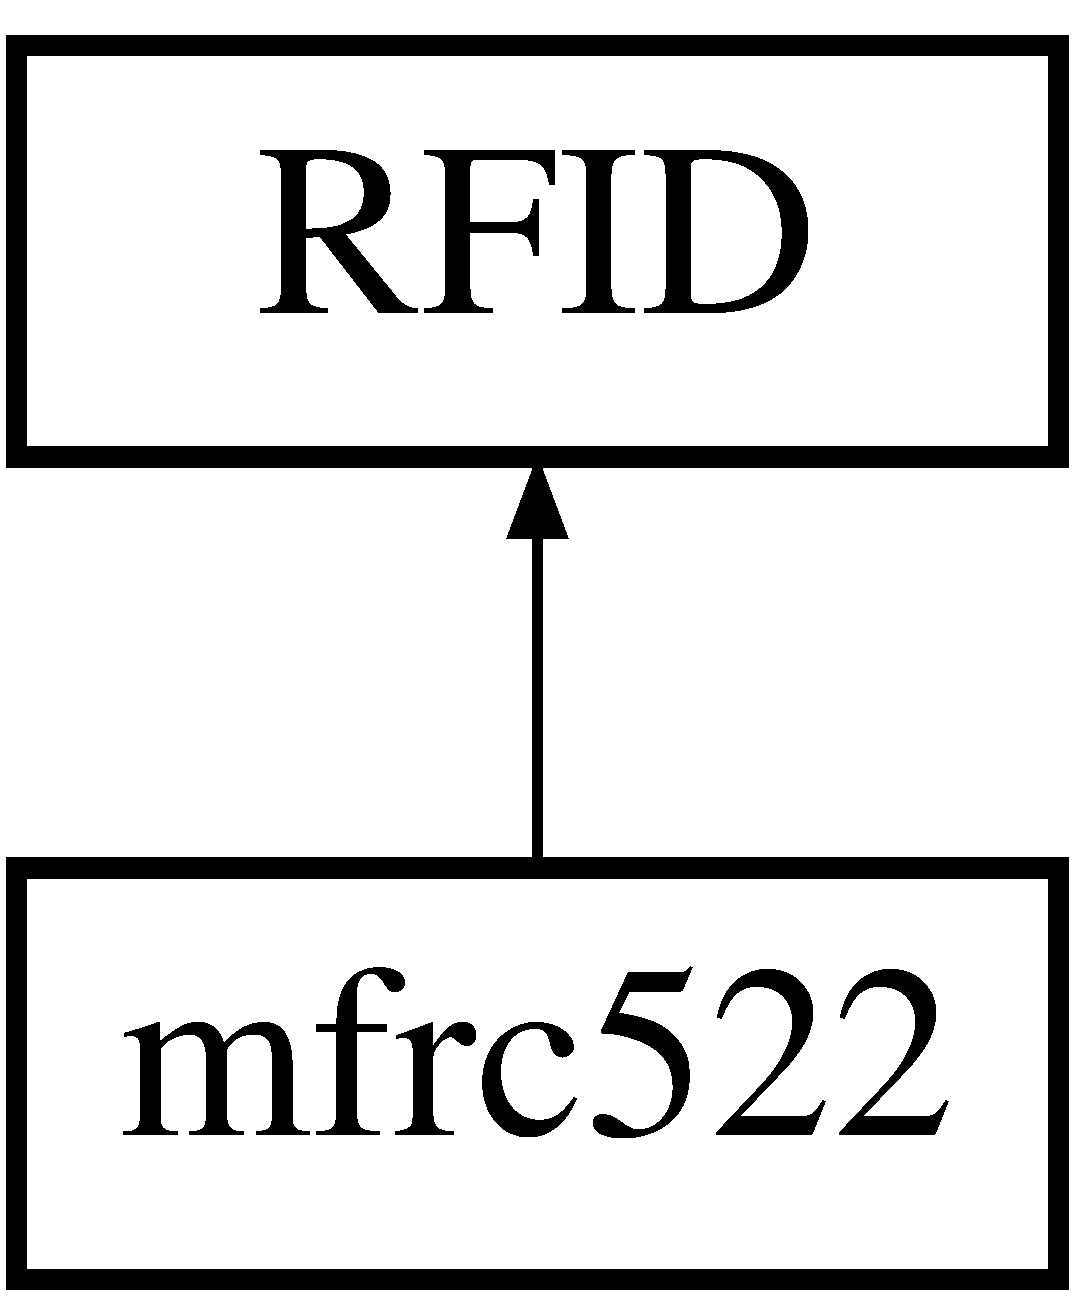
\includegraphics[height=2.000000cm]{class_r_f_i_d}
\end{center}
\end{figure}
\subsection*{Public Member Functions}
\begin{DoxyCompactItemize}
\item 
\hyperlink{class_r_f_i_d_ad893852fc8a7c6a975a42cf3db951857}{R\+F\+ID} (hwlib\+::spi\+\_\+bus\+\_\+bit\+\_\+banged\+\_\+sclk\+\_\+mosi\+\_\+miso \&spi, hwlib\+::target\+::pin\+\_\+out \&S\+DA)
\begin{DoxyCompactList}\small\item\em Default constructor. \end{DoxyCompactList}\item 
virtual void \hyperlink{class_r_f_i_d_a8b244d38edcafaeb06637dbf33b5656f}{init} ()=0
\begin{DoxyCompactList}\small\item\em Initialize the \hyperlink{class_r_f_i_d}{R\+F\+ID} reader. \end{DoxyCompactList}\item 
virtual void \hyperlink{class_r_f_i_d_a3f1242db1a6bb7b57d6bfb7111d1fadd}{reset} (byte addr, byte reset\+Value)
\begin{DoxyCompactList}\small\item\em Soft reset the reader. \end{DoxyCompactList}\item 
virtual void \hyperlink{class_r_f_i_d_a44da5195bf18d4882f1b691904e993b6}{spi\+Write} (byte reg, byte value)
\begin{DoxyCompactList}\small\item\em Write values to the \hyperlink{classmfrc522}{mfrc522}. \end{DoxyCompactList}\item 
virtual byte \hyperlink{class_r_f_i_d_ac9d2c7f3589feef21aba37a95354c6c2}{spi\+Read} (byte addr)
\begin{DoxyCompactList}\small\item\em Read values from \hyperlink{class_r_f_i_d}{R\+F\+ID} reader. \end{DoxyCompactList}\item 
virtual void \hyperlink{class_r_f_i_d_af8a78df3f2b79c1ffc8ea660693f43ec}{set\+Bit\+Mask} (byte addr, byte mask)
\begin{DoxyCompactList}\small\item\em Set a bitmask. \end{DoxyCompactList}\item 
virtual void \hyperlink{class_r_f_i_d_afa2560b026553dac1f6aa20d17f47438}{clear\+Bit\+Mask} (byte addr, byte mask)
\begin{DoxyCompactList}\small\item\em Clear a bitmask. \end{DoxyCompactList}\item 
virtual void \hyperlink{class_r_f_i_d_ad44955169cde018c9673ae5073fcac24}{to\+Card} (byte value, byte $\ast$send\+Data, int len\+Send\+Data, byte $\ast$card\+Ret\+Value, byte $\ast$back\+Data)=0
\begin{DoxyCompactList}\small\item\em Send data to tag. \end{DoxyCompactList}\item 
virtual void \hyperlink{class_r_f_i_d_a7e02863bc0f1f117b05d72f9063497f7}{wait\+For\+Card\+ID} (byte $\ast$ID, int len\+ID)=0
\begin{DoxyCompactList}\small\item\em return a tag U\+ID \end{DoxyCompactList}\end{DoxyCompactItemize}
\subsection*{Protected Attributes}
\begin{DoxyCompactItemize}
\item 
hwlib\+::spi\+\_\+bus\+\_\+bit\+\_\+banged\+\_\+sclk\+\_\+mosi\+\_\+miso \& {\bfseries spi}\hypertarget{class_r_f_i_d_ad2de95fbca075609eb41fa8d27d96077}{}\label{class_r_f_i_d_ad2de95fbca075609eb41fa8d27d96077}

\item 
hwlib\+::target\+::pin\+\_\+out \& {\bfseries S\+DA}\hypertarget{class_r_f_i_d_a4367d5ca78409b651a56920886e8fac2}{}\label{class_r_f_i_d_a4367d5ca78409b651a56920886e8fac2}

\end{DoxyCompactItemize}


\subsection{Detailed Description}
\hyperlink{class_r_f_i_d}{R\+F\+ID} superclass. 

This is a superclass for \hyperlink{class_r_f_i_d}{R\+F\+ID} readers. It contains some basic functions an \hyperlink{class_r_f_i_d}{R\+F\+ID} reader needs to operate. Some of the functions in this class are abstract because the implementation will be different for different \hyperlink{class_r_f_i_d}{R\+F\+ID} readers. 

\subsection{Constructor \& Destructor Documentation}
\index{R\+F\+ID@{R\+F\+ID}!R\+F\+ID@{R\+F\+ID}}
\index{R\+F\+ID@{R\+F\+ID}!R\+F\+ID@{R\+F\+ID}}
\subsubsection[{\texorpdfstring{R\+F\+I\+D(hwlib\+::spi\+\_\+bus\+\_\+bit\+\_\+banged\+\_\+sclk\+\_\+mosi\+\_\+miso \&spi, hwlib\+::target\+::pin\+\_\+out \&\+S\+D\+A)}{RFID(hwlib::spi_bus_bit_banged_sclk_mosi_miso &spi, hwlib::target::pin_out &SDA)}}]{\setlength{\rightskip}{0pt plus 5cm}R\+F\+I\+D\+::\+R\+F\+ID (
\begin{DoxyParamCaption}
\item[{hwlib\+::spi\+\_\+bus\+\_\+bit\+\_\+banged\+\_\+sclk\+\_\+mosi\+\_\+miso \&}]{spi, }
\item[{hwlib\+::target\+::pin\+\_\+out \&}]{S\+DA}
\end{DoxyParamCaption}
)}\hypertarget{class_r_f_i_d_ad893852fc8a7c6a975a42cf3db951857}{}\label{class_r_f_i_d_ad893852fc8a7c6a975a42cf3db951857}


Default constructor. 

This constructor takes a spi bus and a select pin as parameter. It sets the protected variables using these parameters. The protected variables can be used by the \hyperlink{class_r_f_i_d}{R\+F\+ID} class or any other class that inherits the \hyperlink{class_r_f_i_d}{R\+F\+ID} class. 

\subsection{Member Function Documentation}
\index{R\+F\+ID@{R\+F\+ID}!clear\+Bit\+Mask@{clear\+Bit\+Mask}}
\index{clear\+Bit\+Mask@{clear\+Bit\+Mask}!R\+F\+ID@{R\+F\+ID}}
\subsubsection[{\texorpdfstring{clear\+Bit\+Mask(byte addr, byte mask)}{clearBitMask(byte addr, byte mask)}}]{\setlength{\rightskip}{0pt plus 5cm}void R\+F\+I\+D\+::clear\+Bit\+Mask (
\begin{DoxyParamCaption}
\item[{byte}]{addr, }
\item[{byte}]{mask}
\end{DoxyParamCaption}
)\hspace{0.3cm}{\ttfamily [virtual]}}\hypertarget{class_r_f_i_d_afa2560b026553dac1f6aa20d17f47438}{}\label{class_r_f_i_d_afa2560b026553dac1f6aa20d17f47438}


Clear a bitmask. 

This function turns certain bits of in the specified address and keeps the rest the same. It dus this by reading the specified register and then using a and operator on the returned value. The mask itself needs to be inverted to be correct. \index{R\+F\+ID@{R\+F\+ID}!init@{init}}
\index{init@{init}!R\+F\+ID@{R\+F\+ID}}
\subsubsection[{\texorpdfstring{init()=0}{init()=0}}]{\setlength{\rightskip}{0pt plus 5cm}virtual void R\+F\+I\+D\+::init (
\begin{DoxyParamCaption}
{}
\end{DoxyParamCaption}
)\hspace{0.3cm}{\ttfamily [pure virtual]}}\hypertarget{class_r_f_i_d_a8b244d38edcafaeb06637dbf33b5656f}{}\label{class_r_f_i_d_a8b244d38edcafaeb06637dbf33b5656f}


Initialize the \hyperlink{class_r_f_i_d}{R\+F\+ID} reader. 

This function is meant to initialize the \hyperlink{class_r_f_i_d}{R\+F\+ID} reader. It can be used to set any settings needed to succesfully read an \hyperlink{class_r_f_i_d}{R\+F\+ID} tag. The function will have a different meaning for every \hyperlink{class_r_f_i_d}{R\+F\+ID} reader. It will be dependent on the company who made the \hyperlink{class_r_f_i_d}{R\+F\+ID} reader. 

Implemented in \hyperlink{classmfrc522_ac0a0cf7f16b98c37826ce0e160877269}{mfrc522}.

\index{R\+F\+ID@{R\+F\+ID}!reset@{reset}}
\index{reset@{reset}!R\+F\+ID@{R\+F\+ID}}
\subsubsection[{\texorpdfstring{reset(byte addr, byte reset\+Value)}{reset(byte addr, byte resetValue)}}]{\setlength{\rightskip}{0pt plus 5cm}void R\+F\+I\+D\+::reset (
\begin{DoxyParamCaption}
\item[{byte}]{addr, }
\item[{byte}]{reset\+Value}
\end{DoxyParamCaption}
)\hspace{0.3cm}{\ttfamily [virtual]}}\hypertarget{class_r_f_i_d_a3f1242db1a6bb7b57d6bfb7111d1fadd}{}\label{class_r_f_i_d_a3f1242db1a6bb7b57d6bfb7111d1fadd}


Soft reset the reader. 

This funtion is meant to make a soft reset easy to do. The register that has to be set will be different for every \hyperlink{class_r_f_i_d}{R\+F\+ID} reader. But in the end they all have to send some value to an register address. \index{R\+F\+ID@{R\+F\+ID}!set\+Bit\+Mask@{set\+Bit\+Mask}}
\index{set\+Bit\+Mask@{set\+Bit\+Mask}!R\+F\+ID@{R\+F\+ID}}
\subsubsection[{\texorpdfstring{set\+Bit\+Mask(byte addr, byte mask)}{setBitMask(byte addr, byte mask)}}]{\setlength{\rightskip}{0pt plus 5cm}void R\+F\+I\+D\+::set\+Bit\+Mask (
\begin{DoxyParamCaption}
\item[{byte}]{addr, }
\item[{byte}]{mask}
\end{DoxyParamCaption}
)\hspace{0.3cm}{\ttfamily [virtual]}}\hypertarget{class_r_f_i_d_af8a78df3f2b79c1ffc8ea660693f43ec}{}\label{class_r_f_i_d_af8a78df3f2b79c1ffc8ea660693f43ec}


Set a bitmask. 

This function reads the given address and then turns the mask bits in the return value on. After doing this it sends back the new data to the same adress. \index{R\+F\+ID@{R\+F\+ID}!spi\+Read@{spi\+Read}}
\index{spi\+Read@{spi\+Read}!R\+F\+ID@{R\+F\+ID}}
\subsubsection[{\texorpdfstring{spi\+Read(byte addr)}{spiRead(byte addr)}}]{\setlength{\rightskip}{0pt plus 5cm}byte R\+F\+I\+D\+::spi\+Read (
\begin{DoxyParamCaption}
\item[{byte}]{addr}
\end{DoxyParamCaption}
)\hspace{0.3cm}{\ttfamily [virtual]}}\hypertarget{class_r_f_i_d_ac9d2c7f3589feef21aba37a95354c6c2}{}\label{class_r_f_i_d_ac9d2c7f3589feef21aba37a95354c6c2}


Read values from \hyperlink{class_r_f_i_d}{R\+F\+ID} reader. 

This function reads values from a register that has been specified when the function is beeing called. Because the adresses from the spi interface need a 1 on the M\+SB spot to identify that information is beeing read, the address is beeing changed using a or operator (addr $\vert$ 0x80). After this two byte arrays are created. One for the outgoing adresses and the other one for the received information. The function returns the received value as one byte. \index{R\+F\+ID@{R\+F\+ID}!spi\+Write@{spi\+Write}}
\index{spi\+Write@{spi\+Write}!R\+F\+ID@{R\+F\+ID}}
\subsubsection[{\texorpdfstring{spi\+Write(byte reg, byte value)}{spiWrite(byte reg, byte value)}}]{\setlength{\rightskip}{0pt plus 5cm}void R\+F\+I\+D\+::spi\+Write (
\begin{DoxyParamCaption}
\item[{byte}]{reg, }
\item[{byte}]{value}
\end{DoxyParamCaption}
)\hspace{0.3cm}{\ttfamily [virtual]}}\hypertarget{class_r_f_i_d_a44da5195bf18d4882f1b691904e993b6}{}\label{class_r_f_i_d_a44da5195bf18d4882f1b691904e993b6}


Write values to the \hyperlink{classmfrc522}{mfrc522}. 

This function writes values to the \hyperlink{class_r_f_i_d}{R\+F\+ID} reader using the bit banged spi bus from the hwlib namespace. It takes a register to write the value to and the value itself. It puts these bytes in a byte array. The byte array gets send to the spi but from the hwlib namespace as 2 bytes of information that have to be send. \index{R\+F\+ID@{R\+F\+ID}!to\+Card@{to\+Card}}
\index{to\+Card@{to\+Card}!R\+F\+ID@{R\+F\+ID}}
\subsubsection[{\texorpdfstring{to\+Card(byte value, byte $\ast$send\+Data, int len\+Send\+Data, byte $\ast$card\+Ret\+Value, byte $\ast$back\+Data)=0}{toCard(byte value, byte *sendData, int lenSendData, byte *cardRetValue, byte *backData)=0}}]{\setlength{\rightskip}{0pt plus 5cm}virtual void R\+F\+I\+D\+::to\+Card (
\begin{DoxyParamCaption}
\item[{byte}]{value, }
\item[{byte $\ast$}]{send\+Data, }
\item[{int}]{len\+Send\+Data, }
\item[{byte $\ast$}]{card\+Ret\+Value, }
\item[{byte $\ast$}]{back\+Data}
\end{DoxyParamCaption}
)\hspace{0.3cm}{\ttfamily [pure virtual]}}\hypertarget{class_r_f_i_d_ad44955169cde018c9673ae5073fcac24}{}\label{class_r_f_i_d_ad44955169cde018c9673ae5073fcac24}


Send data to tag. 

This function is meant to be used to send data to the \hyperlink{class_r_f_i_d}{R\+F\+ID} tag and if necessary return the data. It takes data to send and the length of this data. There also need to be given 2 byte arrays to return certain data. The first is meant to return a status for the data. So if there is an error it will be in the card\+Ret\+Value array on index 0. The second item in the first array is the length of back\+Data. Back\+Data will contain every bit of data the \hyperlink{class_r_f_i_d}{R\+F\+ID} reader read off the tag. 

Implemented in \hyperlink{classmfrc522_a6801b8481392f6310b40a6893f6544c2}{mfrc522}.

\index{R\+F\+ID@{R\+F\+ID}!wait\+For\+Card\+ID@{wait\+For\+Card\+ID}}
\index{wait\+For\+Card\+ID@{wait\+For\+Card\+ID}!R\+F\+ID@{R\+F\+ID}}
\subsubsection[{\texorpdfstring{wait\+For\+Card\+I\+D(byte $\ast$\+I\+D, int len\+I\+D)=0}{waitForCardID(byte *ID, int lenID)=0}}]{\setlength{\rightskip}{0pt plus 5cm}virtual void R\+F\+I\+D\+::wait\+For\+Card\+ID (
\begin{DoxyParamCaption}
\item[{byte $\ast$}]{ID, }
\item[{int}]{len\+ID}
\end{DoxyParamCaption}
)\hspace{0.3cm}{\ttfamily [pure virtual]}}\hypertarget{class_r_f_i_d_a7e02863bc0f1f117b05d72f9063497f7}{}\label{class_r_f_i_d_a7e02863bc0f1f117b05d72f9063497f7}


return a tag U\+ID 

This function waits for a tag to be held against the \hyperlink{class_r_f_i_d}{R\+F\+ID} reader. It returns the U\+ID of that tag. It returns the U\+ID using the byte array ID. The implementation will be different for different \hyperlink{class_r_f_i_d}{R\+F\+ID} readers. 

Implemented in \hyperlink{classmfrc522_a18665350caf822a716f2a72674a21647}{mfrc522}.



The documentation for this class was generated from the following files\+:\begin{DoxyCompactItemize}
\item 
\hyperlink{_r_f_i_d_8hpp}{R\+F\+I\+D.\+hpp}\item 
\hyperlink{_r_f_i_d_8cpp}{R\+F\+I\+D.\+cpp}\end{DoxyCompactItemize}

\hypertarget{classservo}{}\section{servo Class Reference}
\label{classservo}\index{servo@{servo}}


Servo controll class.  




{\ttfamily \#include $<$servo.\+hpp$>$}

Inheritance diagram for servo\+:\begin{figure}[H]
\begin{center}
\leavevmode
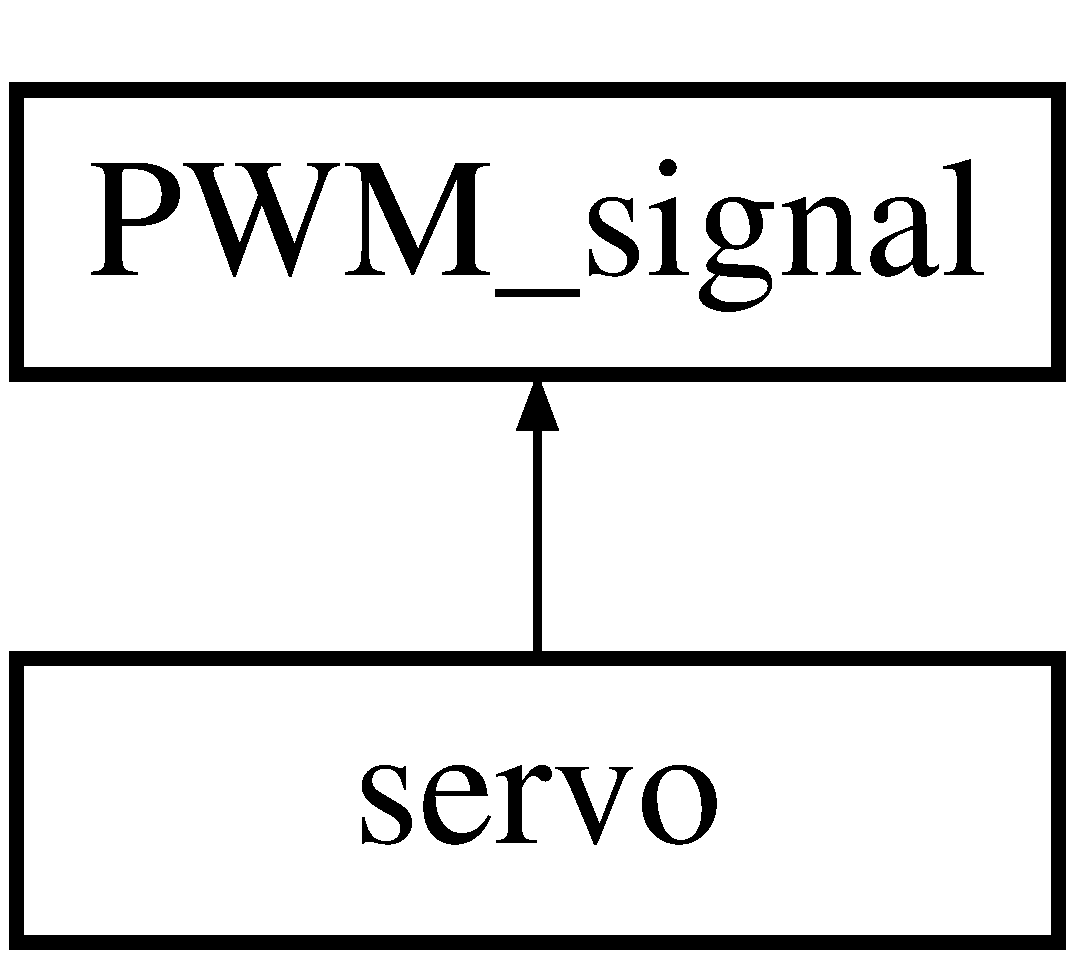
\includegraphics[height=2.000000cm]{classservo}
\end{center}
\end{figure}
\subsection*{Public Member Functions}
\begin{DoxyCompactItemize}
\item 
\hyperlink{classservo_a99c6a39c75cd91b8b2c498cca77d7239}{servo} (hwlib\+::target\+::pin\+\_\+out \&pwm\+Pin)
\begin{DoxyCompactList}\small\item\em Default constructor. \end{DoxyCompactList}\item 
void \hyperlink{classservo_ac0fa39642e5294471844d1fd56e9fec5}{turn\+Degrees} (int degrees)
\begin{DoxyCompactList}\small\item\em Turn the servo to a amount of degrees. \end{DoxyCompactList}\end{DoxyCompactItemize}


\subsection{Detailed Description}
Servo controll class. 

This class is meant to act as a decorator class to the \hyperlink{class_p_w_m__signal}{P\+W\+M\+\_\+signal} class. The idea is that it takes the pulse function and modifies it to send the correct signal for a servo. 

\subsection{Constructor \& Destructor Documentation}
\index{servo@{servo}!servo@{servo}}
\index{servo@{servo}!servo@{servo}}
\subsubsection[{\texorpdfstring{servo(hwlib\+::target\+::pin\+\_\+out \&pwm\+Pin)}{servo(hwlib::target::pin_out &pwmPin)}}]{\setlength{\rightskip}{0pt plus 5cm}servo\+::servo (
\begin{DoxyParamCaption}
\item[{hwlib\+::target\+::pin\+\_\+out \&}]{pwm\+Pin}
\end{DoxyParamCaption}
)}\hypertarget{classservo_a99c6a39c75cd91b8b2c498cca77d7239}{}\label{classservo_a99c6a39c75cd91b8b2c498cca77d7239}


Default constructor. 

This constructor gets a reference to pin on the Arduino Due. This pin is used to set up the P\+WM signal. 

\subsection{Member Function Documentation}
\index{servo@{servo}!turn\+Degrees@{turn\+Degrees}}
\index{turn\+Degrees@{turn\+Degrees}!servo@{servo}}
\subsubsection[{\texorpdfstring{turn\+Degrees(int degrees)}{turnDegrees(int degrees)}}]{\setlength{\rightskip}{0pt plus 5cm}void servo\+::turn\+Degrees (
\begin{DoxyParamCaption}
\item[{int}]{degrees}
\end{DoxyParamCaption}
)}\hypertarget{classservo_ac0fa39642e5294471844d1fd56e9fec5}{}\label{classservo_ac0fa39642e5294471844d1fd56e9fec5}


Turn the servo to a amount of degrees. 

This function get an amount of degrees and then it calculates the wait time. This wait time is beeing given to the pulse function. It also makes sure the servo gets more then one pulse to make sure it has enough time to turn to the set amount of degrees. 

The documentation for this class was generated from the following files\+:\begin{DoxyCompactItemize}
\item 
D\+:/programmeren/\+Projecten/\+I\+P\+A\+S-\/project/rfid\+\_\+keypad\+\_\+lock/\+Finished\+\_\+librarys/\hyperlink{servo_8hpp}{servo.\+hpp}\item 
D\+:/programmeren/\+Projecten/\+I\+P\+A\+S-\/project/rfid\+\_\+keypad\+\_\+lock/\+Finished\+\_\+librarys/servo.\+cpp\end{DoxyCompactItemize}

\chapter{File Documentation}
\hypertarget{matrix_keypad_8hpp}{}\section{D\+:/programmeren/\+Projecten/\+I\+P\+A\+S-\/project/rfid\+\_\+keypad\+\_\+lock/\+Finished\+\_\+librarys/matrix\+Keypad.hpp File Reference}
\label{matrix_keypad_8hpp}\index{D\+:/programmeren/\+Projecten/\+I\+P\+A\+S-\/project/rfid\+\_\+keypad\+\_\+lock/\+Finished\+\_\+librarys/matrix\+Keypad.\+hpp@{D\+:/programmeren/\+Projecten/\+I\+P\+A\+S-\/project/rfid\+\_\+keypad\+\_\+lock/\+Finished\+\_\+librarys/matrix\+Keypad.\+hpp}}
{\ttfamily \#include \char`\"{}hwlib.\+hpp\char`\"{}}\\*
\subsection*{Classes}
\begin{DoxyCompactItemize}
\item 
class \hyperlink{classmatrix_keypad}{matrix\+Keypad}
\begin{DoxyCompactList}\small\item\em Obtain pressed keys from a keypad. \end{DoxyCompactList}\end{DoxyCompactItemize}

\hypertarget{mfrc522_8hpp}{}\section{mfrc522.\+hpp File Reference}
\label{mfrc522_8hpp}\index{mfrc522.\+hpp@{mfrc522.\+hpp}}
{\ttfamily \#include \char`\"{}hwlib.\+hpp\char`\"{}}\\*
{\ttfamily \#include \char`\"{}R\+F\+I\+D.\+hpp\char`\"{}}\\*
\subsection*{Classes}
\begin{DoxyCompactItemize}
\item 
class \hyperlink{classmfrc522}{mfrc522}
\begin{DoxyCompactList}\small\item\em Reading \hyperlink{class_r_f_i_d}{R\+F\+ID} tags with \hyperlink{classmfrc522}{mfrc522}. \end{DoxyCompactList}\end{DoxyCompactItemize}

\hypertarget{_p_w_m__signal_8hpp}{}\section{P\+W\+M\+\_\+signal.\+hpp File Reference}
\label{_p_w_m__signal_8hpp}\index{P\+W\+M\+\_\+signal.\+hpp@{P\+W\+M\+\_\+signal.\+hpp}}
{\ttfamily \#include \char`\"{}hwlib.\+hpp\char`\"{}}\\*
\subsection*{Classes}
\begin{DoxyCompactItemize}
\item 
class \hyperlink{class_p_w_m__signal}{P\+W\+M\+\_\+signal}
\begin{DoxyCompactList}\small\item\em Basic P\+WM signal. \end{DoxyCompactList}\end{DoxyCompactItemize}

\hypertarget{_r_f_i_d_8cpp}{}\section{R\+F\+I\+D.\+cpp File Reference}
\label{_r_f_i_d_8cpp}\index{R\+F\+I\+D.\+cpp@{R\+F\+I\+D.\+cpp}}
{\ttfamily \#include \char`\"{}R\+F\+I\+D.\+hpp\char`\"{}}\\*

\hypertarget{_r_f_i_d_8hpp}{}\section{R\+F\+I\+D.\+hpp File Reference}
\label{_r_f_i_d_8hpp}\index{R\+F\+I\+D.\+hpp@{R\+F\+I\+D.\+hpp}}
{\ttfamily \#include \char`\"{}hwlib.\+hpp\char`\"{}}\\*
\subsection*{Classes}
\begin{DoxyCompactItemize}
\item 
class \hyperlink{class_r_f_i_d}{R\+F\+ID}
\begin{DoxyCompactList}\small\item\em \hyperlink{class_r_f_i_d}{R\+F\+ID} superclass. \end{DoxyCompactList}\end{DoxyCompactItemize}

\hypertarget{servo_8hpp}{}\section{servo.\+hpp File Reference}
\label{servo_8hpp}\index{servo.\+hpp@{servo.\+hpp}}
{\ttfamily \#include \char`\"{}P\+W\+M\+\_\+signal.\+hpp\char`\"{}}\\*
{\ttfamily \#include \char`\"{}hwlib.\+hpp\char`\"{}}\\*
\subsection*{Classes}
\begin{DoxyCompactItemize}
\item 
class \hyperlink{classservo}{servo}
\begin{DoxyCompactList}\small\item\em Servo controll class. \end{DoxyCompactList}\end{DoxyCompactItemize}
\subsection*{Macros}
\begin{DoxyCompactItemize}
\item 
\#define {\bfseries M\+A\+X\+\_\+\+D\+E\+G\+R\+E\+ES}~249\hypertarget{servo_8hpp_a4ba510f21f53f375dd98267c4a644281}{}\label{servo_8hpp_a4ba510f21f53f375dd98267c4a644281}

\item 
\#define {\bfseries M\+I\+N\+\_\+\+D\+E\+G\+R\+E\+ES}~0\hypertarget{servo_8hpp_a0433cf7215e086e910d2fc9f84c25e79}{}\label{servo_8hpp_a0433cf7215e086e910d2fc9f84c25e79}

\end{DoxyCompactItemize}

%--- End generated contents ---

% Index
\backmatter
\newpage
\phantomsection
\clearemptydoublepage
\addcontentsline{toc}{chapter}{Index}
\printindex

\end{document}
